\chapter{Conclusion and Outlook}


\section{Using Incoherent Imaging for Online Beam Diagnostic}



The posibility to run an IDI setup in parallel with other detectors would allow for a combination of IDI with CDI

Larger detectors

Short pulses

Element specific 


Even just the ability to image to focal volume might be an useful diagnostic tool in certain experiments


An avenue for improvement is subpixel resolution of the photon hits and better usage of the varying XXX of the detector to increase the resolution in the reconstruction, as this is currenly limited by the computional intensity to calulate the correlations at higher resolution.


\begin{figure}
	\centering
	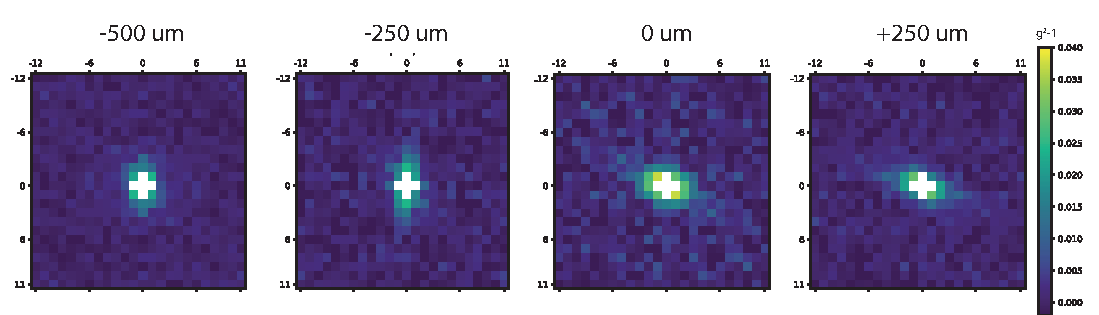
\includegraphics[width=\linewidth]{images/lv65_vanadium.pdf}
	\label{fig:outlook_vanadium}
	\caption[Focus finding using IDI]{Preliminary results of the $g^2(\vec{q})$ calculation of the fluorescence of a 4\,um vanadium foil, placed at 4 different positions along the x-ray beam at the CXI experimental hutch (LCLS, running in an experimental configuration for short pulse duration under 1\,fs \cite{argosecond}) using the "100 nm" KB focusing (optimal theoretical focus size 90\,nm x 150\,nm, theoretical beam divergence 2 mrad x 1 mrad) on one tile of a Jungfrau detector (75\,um pixelsize, placed 480\,mm downstream of the sample). Shown are averages over ~2000 shots with minimal shot based filtering. The position captioned "0" was determined during the experiment as the focus based on these results, the other positions are 250\,um and 500\,um further downstream and 250\,um upstream (position determined as focus by imprints).  Some astigmatism is visible.}
\end{figure}

\section{Experimental Improvements}



\begin{figure}
	\centering
	\begin{subfigure}[b]{0.50\textwidth}
	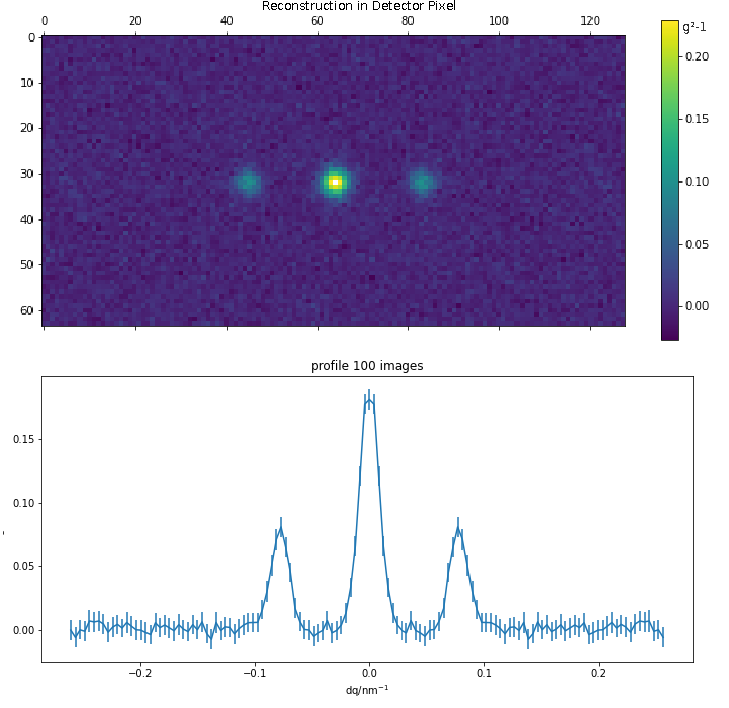
\includegraphics[width=\linewidth]{images/lv65simA.pdf}
	\caption{Nano-Grating}
	\label{fig:outlook_grating}
\end{subfigure}
\begin{subfigure}[b]{0.37\textwidth}
	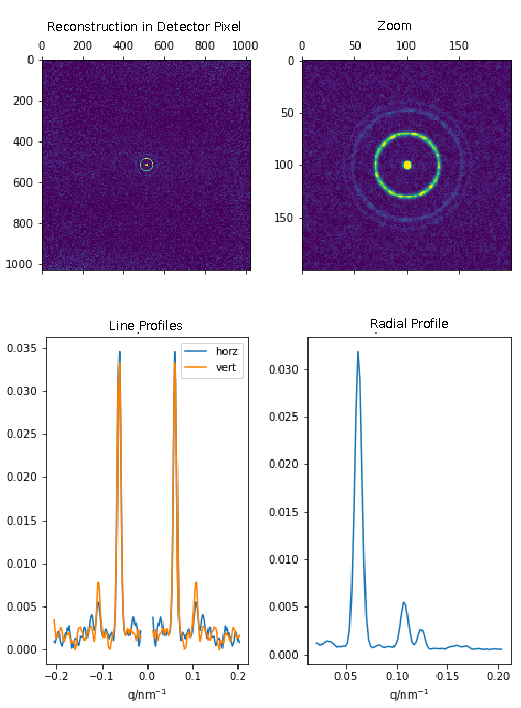
\includegraphics[width=\linewidth]{images/lv65simB.pdf}
	\caption{AAO Membranes}
	\label{fig:outlook_aao}
\end{subfigure}
\caption[Simulations in Preparation of LV65 Experiment]{Examples of simulations performed with the tools developed in this thesis in preparation of an additional experiment (LV65) at the LCLS free electron laser.}
\end{figure}

Upcoming experiment using sub-1\,fs pulse length as LCLS. 
For this experiment, two new, signal optimized samples were chosen: Anodic Aluminum Oxide (AAO) membranes with regular spaced XX pores, with are filled with Nickel or Vanadium using atomic layer deposition, creating an array of hexagonal placed  500\,nm long cylinders. As the order of the self-organizing pores is smaller than the area used in the experiment, the simulated reconstruction shows rings (\fref{fig:outlook_aao}). Using realistic simulation parameters, XXX images should suffice to reach a SNR of XXX.
The other sample is will be a litographically procuced gratings with a pitches of XXX (simulation shown in \fref{fig:outlook_grating}.). Both samples combine the advantes of a single crystal sample (namely intense features) while providing more signal and requiring less accessible reciprocal space. 


Furthermore, for the randomly in plane oriented pores, the SNR might be improved by considering the polar correlations in the single image reconstructions as described in XXX


